Nachdem auf dem Sand trotz unseres Protests die zwei Poolräume C111 und F121 geschlossen wurden und damit sich die Anzahl der studentischen Arbeitsräume immer weiter verringert konnten wir mit unserer Unterschriftenaktion doch einige Verbesserungen erreichen. Zum einen haben wir die Zusage bekommen, dass Studierende die Seminarräume außerhalb der Belegungszeiten zum Lernen und Arbeiten nutzen können. Hierzu haben wir für euch eine Übersicht der dauerhaften Belegungen erstellt. Die Raumbelegung ist auch an unserem Aushang vor dem Fachschaftszimmer und auf unserer Website\footnote{http://www.fsi.uni-tuebingen.de/studium/raumplaene} einsehbar.\\
Desweiteren wurde der studentische Arbeitsraum C119 mit zwei Rechnern und einem Drucker ausgestattet, sodass auch weiterhin das Drucken von Übungsblättern und Abgaben möglich ist.
Außerdem haben wir von der Fachbereichsleitung die Zusage bekommen, dass die Institutsbibliothek mit einem elektronischen Öffnungssystem versehen wird. Mit diesem wird es für alle Informatikstudierende möglich sein, auch außerhalb der Öffnungszeiten, in die Bibliothek zu kommen. Dort sollen zudem die Arbeitsplätze weiter ausgebaut werden, um den Wegfall der Poolräume zu kompensieren.

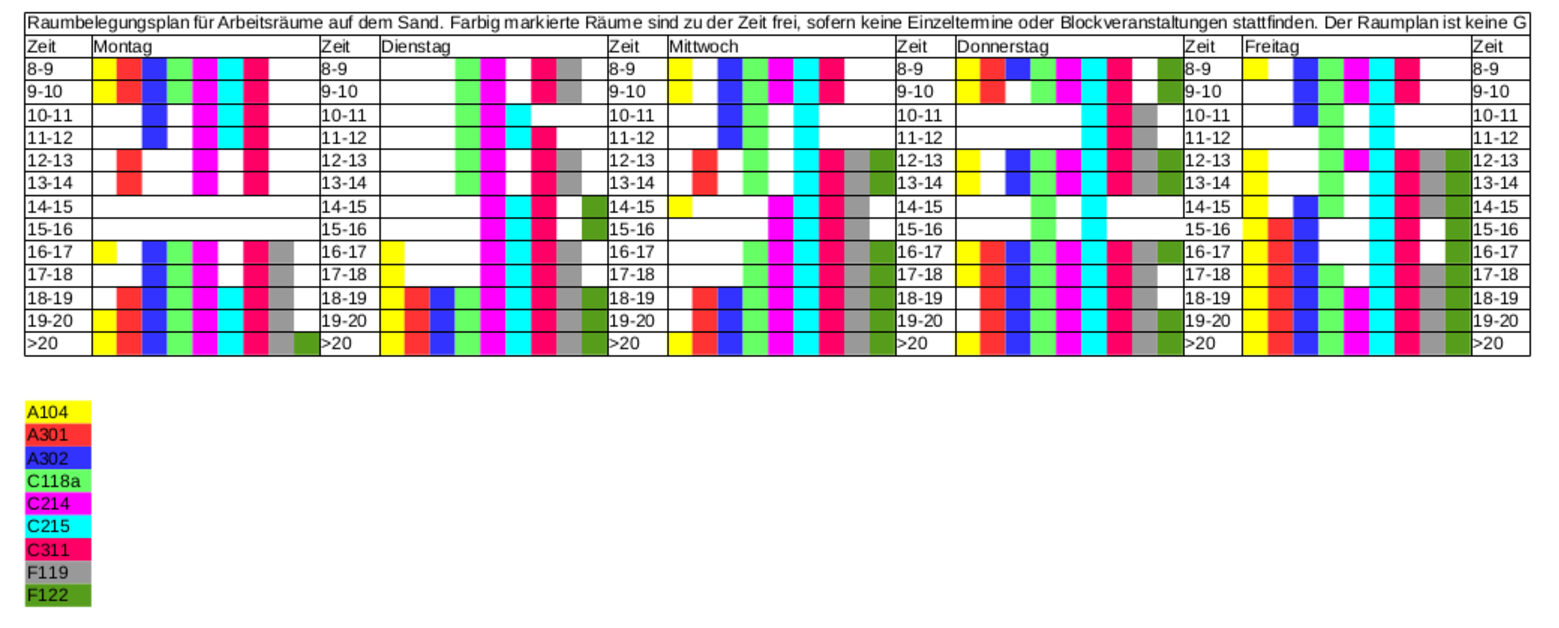
\includegraphics[width=\textwidth]{content/pictures/Raumplan.pdf}
\newpage